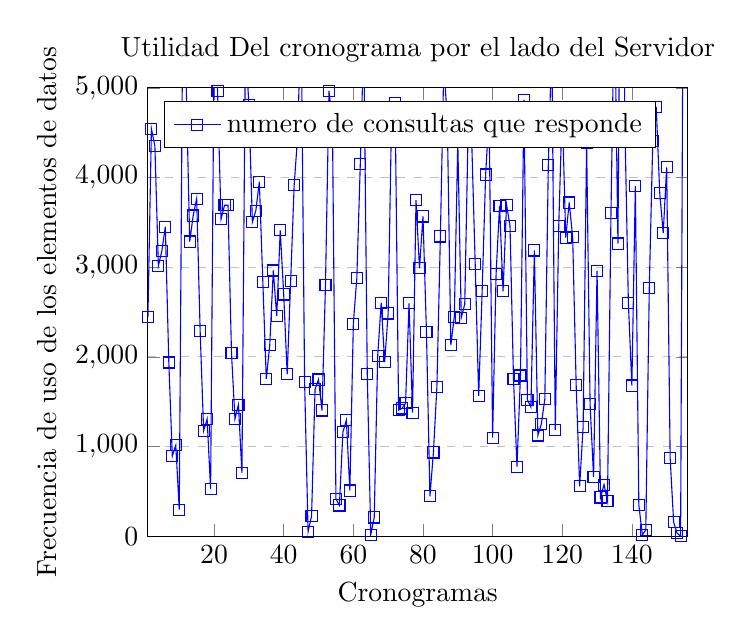
\begin{tikzpicture}
\begin{axis}[
    title={Utilidad Del cronograma por el lado del Servidor},
    xlabel={Cronogramas},
    ylabel={Frecuencia de uso de los elementos de datos},
    xmin=1, xmax=156,
    ymin=0, ymax=5000,
    xtick={},
    ytick={},
    legend pos=north west,
    ymajorgrids=true,
    grid style=dashed,
]

\addplot[
    color=blue,
    mark=square,
    ]
    coordinates {
%UTILIDAD TOTAL
%(cronograma, numero cues que usan al cronograma)
(1,2442)
(2,4544)
(3,4351)
(4,3016)
(5,3181)
(6,3452)
(7,1937)
(8,893)
(9,1014)
(10,296)
(11,5827)
(12,5039)
(13,3286)
(14,3576)
(15,3765)
(16,2286)
(17,1177)
(18,1307)
(19,524)
(20,5419)
(21,4968)
(22,3536)
(23,3691)
(24,3691)
(25,2041)
(26,1308)
(27,1467)
(28,705)
(29,5511)
(30,4805)
(31,3502)
(32,3631)
(33,3953)
(34,2838)
(35,1754)
(36,2136)
(37,2963)
(38,2454)
(39,3411)
(40,2696)
(41,1807)
(42,2849)
(43,3913)
(44,4460)
(45,5842)
(46,1724)
(47,51)
(48,223)
(49,1637)
(50,1747)
(51,1402)
(52,2806)
(53,4965)
(54,4609)
(55,415)
(56,343)
(57,1160)
(58,1294)
(59,509)
(60,2370)
(61,2879)
(62,4153)
(63,5561)
(64,1813)
(65,17)
(66,209)
(67,2012)
(68,2603)
(69,1941)
(70,2484)
(71,4742)
(72,4830)
(73,1407)
(74,1425)
(75,1482)
(76,2597)
(77,1377)
(78,3747)
(79,2987)
(80,3566)
(81,2278)
(82,444)
(83,934)
(84,1667)
(85,3343)
(86,5277)
(87,4626)
(88,2130)
(89,2449)
(90,4395)
(91,2437)
(92,2587)
(93,4591)
(94,4409)
(95,3037)
(96,1565)
(97,2737)
(98,4033)
(99,4721)
(100,1099)
(101,2922)
(102,3686)
(103,2731)
(104,3696)
(105,3462)
(106,1757)
(107,775)
(108,1792)
(109,4869)
(110,1523)
(111,1440)
(112,3187)
(113,1123)
(114,1252)
(115,1529)
(116,4137)
(117,5532)
(118,1185)
(119,3463)
(120,4782)
(121,3329)
(122,3721)
(123,3334)
(124,1689)
(125,557)
(126,1216)
(127,4384)
(128,1472)
(129,661)
(130,2960)
(131,432)
(132,575)
(133,392)
(134,3603)
(135,6075)
(136,3264)
(137,8665)
(138,4581)
(139,2600)
(140,1680)
(141,3906)
(142,350)
(143,15)
(144,69)
(145,2768)
(146,4405)
(147,4787)
(148,3830)
(149,3380)
(150,4114)
(151,868)
(152,155)
(153,33)
(154,0)
(155,8820)
(156,5806)
    };
    \legend{numero de consultas que responde}

\end{axis}
\end{tikzpicture}

